% Created 2021-01-24 Sun 22:50
% Intended LaTeX compiler: pdflatex
\documentclass[11pt]{article}
\usepackage[utf8]{inputenc}
\usepackage[T1]{fontenc}
\usepackage{graphicx}
\usepackage{grffile}
\usepackage{longtable}
\usepackage{wrapfig}
\usepackage{rotating}
\usepackage[normalem]{ulem}
\usepackage{amsmath}
\usepackage{textcomp}
\usepackage{amssymb}
\usepackage{capt-of}
\usepackage{hyperref}
\usepackage{minted}
\hypersetup{colorlinks=true, linkcolor=black, filecolor=red, urlcolor=blue}
\usepackage[turkish]{babel}
\author{Eren Hatırnaz}
\date{1 Aralık 2019}
\title{Yazılım Gündemi - 19\\\medskip
\large 18 Kasım-1 Aralık 2019}
\hypersetup{
 pdfauthor={Eren Hatırnaz},
 pdftitle={Yazılım Gündemi - 19},
 pdfkeywords={},
 pdfsubject={},
 pdfcreator={Emacs 27.1 (Org mode 9.3)},
 pdflang={Turkish}}
\begin{document}

\maketitle
\tableofcontents \clearpage\shorthandoff{=}

\begin{center}
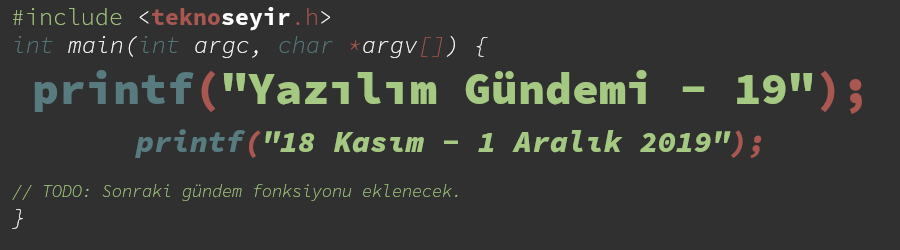
\includegraphics[width=.9\linewidth]{gorseller/yazilim-gundemi-banner.png}
\end{center}

\begin{center}
\href{../18/yazilim-gundemi-18.pdf}{< Önceki Gündem} | \textbf{18 Kasım-1 Aralık 2019} | \href{../20/yazilim-gundemi-20.pdf}{Sonraki Gündem >}

\href{https://teknoseyir.com/blog/yazilim-gundemi-19-18-kasim-1-aralik-2019}{TeknoSeyir'de Oku}
\end{center}

\section{\href{https://www.oyd.org.tr/}{Özgür Yazılım Derneği} kuruldu}
\label{sec:orgb45fa56}
\begin{center}

\includegraphics[height=5cm]{gorseller/ozgur-yazilim-dernegi.jpg}
\end{center}

Özgür Yazılım, Richard Stallman tarafından ortaya atılmış ve topluluk
tarafından geliştirilmiş bir felsefedir. Her ne kadar Richard Stallman'ın
karıştığı son olaylar (\href{../10/yazilim-gundemi-10.pdf}{Yazılım Gündemi - 10}) hoş olmasa da böyle bir felsefeyi
ve akımı başlatması açısından bence önemli bir kişiliktir. Bu felsefe dünya
genelinde Free Software Foundation oluşumu üzerinden tanıtılmaya ve yayılmaya
çalışıyor fakat Türkiye'de de bu konuyu önemseyen kişiler tarafından bir
girişim yapılmış ve Özgür Yazılım Derneği, İstanbul'da kurulmuş. Derneğin web
sitesinden anladığım kadarıyla sanırım dernek yeni kurulmadı, bir süredir var
fakat benim de bu hafta \href{https://teknoseyir.com/haftalik-gundem-degerlendirmesi-2019-48}{Haftalık Gündem Değerlendirmesi 2019/48}'de duyarak
haberdar olduğum bir oluşum oldu.

Derneğin web sitesini incelediğimde 3 üyelik tipinin bulunduğunu öğrendim.
Bunlar şu şekilde:

\begin{quote}
\begin{itemize}
\item Destekçi Üye: Derneğin faaliyetlerine destek olmak amacıyla maddi veya ayni
yardımda bulunan üyelerdir.
\item Üye: Dernek tüzüğünün 5⁄1 fıkrası uyarınca hukuken derneğin üyesi olan,
Genel Kurulu oluşturan, dernek organlarını seçme ve organlarda görev alma
hakkı bulunan üyelerdir.
\item Onur Üyeliği: Derneğin amaçları için çalışmış, toplumda bu konuda saygı
gören ve eserleri ile dernek amaçlarına katkısı bulunmuş kişiler arasından
Genel Kurul kararı ile üyeliğe alınan üyelerdir. Onur üyelerinin aidat
yükümlülüğü ve oy hakları yoktur.
\end{itemize}
\end{quote}

Desteki Üye olmak kategorisinden derneğe katılmak bir SMS uzaklığınızda. OYD
yazıp 8071'e gönderdiğiniz takdirde Özgür Yazılım Derneğine aylık 20TL bağışta
bulunabilir (10 TL için OYD10 yazabilirsiniz) ve sayfada sizden istenen birkaç
bilgiyi sağlayarak Destekçi Üye kaydınızı tamamlayabilirsiniz. Diğer bağış
yöntemleri için \href{https://bagis.oyd.org.tr/}{bu sayfayı} inceleyebilirsiniz.

Derneğin kurulmasında emeği geçen tüm arkadaşları tebrik ederim. Şu an
sektörden biraz uzak olsam da ileride benim de içinde bulunmak istediğim bir
oluşum.
\section{PHP 7.4.0 stabil sürümü \href{https://www.php.net/archive/2019.php\#2019-11-28-1}{yayınlandı}}
\label{sec:org688b94c}
Uzun bir süredir geliştirilmekte olan PHP programlama dilinin 7.4.0 numaralı ve
stabil olan sürümü bu hafta içerisinde yayınlandı. Daha önceki bir yazılım
gündemi yazısında da (bkz: \href{../03/yazilim-gundemi-03.pdf}{Yazılım Gündemi - 3}) paylaştığım üzere PHP 7.4'ün
yayınlanma süreci büyük oranda planladıkları takvime uygun olarak ilerledi ve
tamamlandı. Yine aynı yazılım gündemi yazısında beta süresince olan bazı yeni
özellikleri tanıtmıştım bu yazıda da birkaç farklı özelliğe bakalım:
\subsection{Unpacking inside arrays (Dizi içerisinde dizi açmak)}
\label{sec:org10429f2}
JavaScript ve diğer dillerde spreads ismiyle gördüğümüz bu özellik artık
PHP'de de var. Yani artık bir dizinin elemanlarını başka bir dizinin içerisine
çıkartabileceğiz.
\begin{minted}[breaklines=true,breakanywhere=true,frame=lines, linenos, label=PHP, labelposition=topline, startinline=true]{php}
$parca = ['elma', 'armut'];
$meyveler = ['muz', 'portakal', ...$parca, 'karpuz'];
// dizinin son hali: ['muz', 'portakal', 'elma', 'armut', 'karpuz'];
\end{minted}
\subsection{Numeric literal separator}
\label{sec:org75d8c52}
Daha kolay okunabilmesi için artık sayıları bu şekilde basamaklara
ayırabileceğiz:
\begin{minted}[breaklines=true,breakanywhere=true,frame=lines, linenos, label=PHP, labelposition=topline, startinline=true]{php}
6.674_083e-11; // float
299_792_458;   // decimal
0xCAFE_F00D;   // hexadecimal
0b0101_1111;   // binary
\end{minted}

Elbette eklenen özellikler olduğu gibi değişen ve kullanımdan
kaldırılmaya hazırlanan (deprecate) bazı özellikler de mevcut. Bunlar için \href{https://www.php.net/manual/en/migration74.deprecated.php}{şu
sayayı} ziyaret edebilirsiniz. PHP ile yüklü gelen eklentilerden de şu 3
eklenti artık PHP ile birlikte dağıtılmayacak:
\begin{itemize}
\item \href{https://www.php.net/manual/en/book.ibase.php}{Firebird/Interbase}
\item \href{https://www.php.net/manual/en/book.recode.php}{Recode}
\item \href{https://www.php.net/manual/en/book.wddx.php}{WDDX}
\end{itemize}

Yeni stabil sürümü indirmek isterseniz \href{https://www.php.net/downloads.php}{bu sayfayı} ziyaret edebilirsiniz.
\section{Facebook ve Microsoft'dan uzaktan geliştirme \href{https://developers.facebook.com/blog/post/2019/11/19/facebook-microsoft-partnering-remote-development/}{işbirliği}}
\label{sec:org4df005e}
Malumunuz devir tüm ihtiyaçların bulut bilişim çözümleriyle giderilmeye
çalışıldığı günümüzde konu bize de geldi. Özellikle de son birkaç ayda
duyurulan araçlar ve hizmetlerle de (bkz: \href{../17/yazilim-gundemi-17.pdf}{Yazılım Gündemi - 17}) daha popüler
olan uzaktan geliştirme (Remote Development) konusundan bahsediyorum.
Geçtiğimiz hafta yayınlanan blog yazısı ile birlikte de Microsoft ve Facebook,
Visual Studio Code aracının uzaktan geliştirme özelliklerini iyileştirmek için
birlikte çalışacağı ilan edildi.

Facebook da elbette isteyen kendi rahat ettiği programlama aracını kullanıyor
fakat çoğunluk bir kısım da Facebook'un, Atom editörünü özelleştirerek
çıkardığı Nuclide editörünü kullanıyormuş. Fakat geçtiğimiz yıl bu editörün
açık kaynak sürümünü \href{https://nuclide.io/}{emekliye ayırmışlar}. Microsoft'un Visual Studio Code'a
remote development özelliği eklemeye ve iyileştirmeye başladığından beri bu
özellik Facebook içerisinde çok fazla kullanılıyormuş. Geliştiricilere
getirdiği kolaylıklar ise:
\begin{itemize}
\item Projenin boyutu fark etmeksizin bilgisayarın özelliklerine bağlı kalmadan
istediğin projede zorlanmadan geliştirme yapabilmek,
\item Birbirinden tamamen bağımsız geliştirme ortamları yaratarak projelerin
bağımlılıkları ile ilgili çakışmaları önleyebilmek,
\item Projeler arasında hızlı bir şekilde geçiş yapabilmek ve çalıştırabilmek.
\end{itemize}
Facebook geliştirme ekibi da bu olanaklardan fazlasıyla faydalandıkları için
Microsoft'a bu özelliği iyileştirmek için yardım edecekmiş. Planlanan
iyileştirmelerden yazıda bahsedilmemiş, bakalım ne gibi çalışmalar yapacaklar.

Açıkcası her ne kadar uzaktan geliştirme konusuna pek sıcak bakmasam da
sağladığı kolaylıklar hiç öyle yabana atılır cinsten değil. Özellikle günümüzde
taşınabilir geliştirme ortamları önem kazanmaya başladı. Ben de ileride
aklımdaki sistemi kurabilirsem kendi evimde bu tarz bir uzaktan geliştirme
ortamı yaratmak istiyorum bakalım. Daha önceki bir yazıda sormuştum fakat yeri
gelmişken tekrar sorayım, belki farklı konulara da kapı açabiliriz: Siz uzaktan
geliştirme konusunda ne düşünüyorsunuz? Tercih eder miydiniz? Yorumlar kısmında
konuşalım.
\section{Tüm JetBrains IDE'leri 2019.3 sürümüne güncellendi}
\label{sec:org962afca}
JetBrains, Kotlin programlama dilini üreten firma olmasından ziyade aynı
zamanda çok başarılı ve güçlü programlama araçlarıyla da ünlü bir şirket. Ben
de zamanında çok fazla ürününü kullanmış ve ara ara hala kullanan biri olarak
söyleyebilirim ki gerçekten geliştirici camiasının ihtiyaçlarını çok iyi analiz
eden ve buna göre çözümler üreten bir firmadır. Her neyse konumuza gelelim: Bu
hafta tüm JetBrains IDE'lerine güncellemeler geldi. Benim ilgili olduğum bir
IDE'ye gelen özelliklere birlikte göz atalım:
\newpage
\subsection{\href{https://blog.jetbrains.com/phpstorm/2019/11/phpstorm-2019-3-release/}{PHPStorm 2019.3}}
\label{sec:org71b3ff5}
\begin{center}

\includegraphics[height=3cm]{gorseller/phpstorm-2019.3.png}
\end{center}

\begin{itemize}
\item PHP 7.4 ile gelen bütün özelliklere destek (üstelik deprecate olacakları da
gösteriyor),
\item \href{https://www.php-fig.org/psr/psr-12/}{PSR-12 Standardı} desteği,
\item WSL (Windows Subsystem for Linux) desteği,
\item PHPDoc iyileştirmeleri,
\item Diğer özellikler için alt konu başlığına eklediğim bağlantıya
tıklayabilir ya da \href{https://www.youtube.com/watch?v=h9KGsD87t\_M}{şuradaki videou izleyebilirsiniz}.
\end{itemize}

Diğer IDE güncellemeleri ise şu şekilde:
\begin{itemize}
\item \href{https://blog.jetbrains.com/idea/2019/11/intellij-idea-2019-3-better-performance-and-quality/}{Intellij Idea 2019.3},
\item \href{https://blog.jetbrains.com/webstorm/2019/11/webstorm-2019-3/}{WebStorm 2019.3},
\item \href{https://blog.jetbrains.com/pycharm/2019/11/pycharm-2019-3-release-candidate/}{PyCharm 2019.3},
\item \href{https://blog.jetbrains.com/go/2019/11/29/goland-2019-3/}{GoLand 2019.3},
\item \href{https://blog.jetbrains.com/clion/2019/11/clion-2019-3-release/}{CLion 2019.3},
\item \href{https://blog.jetbrains.com/objc/2019/11/appcode-2019-3-rc/}{AppCode 2013.3 Release Candidate},
\item \href{https://blog.jetbrains.com/datagrip/2019/11/15/datagrip-2019-3-eap-4/}{DataGrid 2019.3 Erken Erişim 4},
\item \href{https://blog.jetbrains.com/ruby/2019/11/rubymine-2019-3-released/}{RubyMine 2019.3},
\item \href{https://blog.jetbrains.com/dotnet/2019/11/18/new-way-commit-introducing-commit-repository-tool-windows-rider-2019-3-eap/}{Rider 2019.3 Erken Erişim}
\end{itemize}
\section{Windows Terminal Preview v0.7 \href{https://devblogs.microsoft.com/commandline/windows-terminal-preview-v0-7-release/}{yayınlandı}}
\label{sec:org05e6c39}
Microsoft'un açık kaynak camiasına açılmasından sonra yaptığı birkaç işi
gerçekten severek takip ediyorum. Bunlardan birisi Visual Studio Code, diğeri
ise Windows Terminal. Her ne kadar geliştirme yapmak için kullandığım dizüstü
bilgisayarımda Windows kullanmasam da oyun bilgisayarı olarak kullandığım
masaüstü sistemimde Windows var ve bazen orada da programlama testleri
yapıyorum. Yeni Windows Terminal'i de WSL (Windows Subsystem for Linux) ile
birlikte kullanıyorum. Bu hafta yeni bir önizleme sürümü olan 0.7 sürümünü
tanıttılar.

\url{gorseller/winterminal-bolme.gif}

Bunların yanında sekmelerin isimlerini özelleştirme ve bazı görsel
iyileştirmeler de katılmış durumda. Ne kadar ön izleme sürümü olsa da, Windows
üzerinde programlama yapan arkadaşlara şiddetle tavsiye ederim.
\section{Yaklaşan Etkinlikler}
\label{sec:org8619f7a}
\begin{longtable}{|p{8cm}|l|l|}
\hline
Etkinlik İsmi & Yeri & Tarihi\\
\hline
\endfirsthead
\multicolumn{3}{l}{Önceki sayfadan devam ediyor} \\
\hline

Etkinlik İsmi & Yeri & Tarihi \\

\hline
\endhead
\hline\multicolumn{3}{r}{Devamı sonraki sayfada} \\
\endfoot
\endlastfoot
\hline
\href{https://www.eventbrite.com/e/bulut-mimarisindeki-yapay-zeka-servisleri-registration-83943492245}{Bulut Mimarisindeki Yapay Zeka Servisleri} & İstanbul & 3 Aralık 19:00\\
\href{https://kommunity.com/devops-turkiye/events/blutv-kubernetes-microservices}{BluTV Kubernetes \& Microservices} & İstanbul & 4 Aralık 18:30\\
\href{https://kommunity.com/software-craftsmanship-turkey/events/yazilim-sektorunde-korku-kaygi-ve-ozguven}{Yazılım Sektöründe Korku, Kaygı ve Özgüven} & İstanbul & 4 Aralık 19:00\\
\href{https://kommunity.com/sovos-foriba-rd/events/microprofile-payara-micro-openshift}{Microprofile \& Payara Micro \& OpenShift} & İstanbul & 5 Aralık 17:00\\
\href{https://btz.org.tr/}{İTÜ İMK 12. Bilişim Teknolojileri Zirvesi} & İstanbul & 6 Aralık 10:00\\
\href{https://www.eventbrite.com/e/python-for-hackers-hacknightsorg-tickets-78151145179}{Python For Hackers} & Ankara & 6 Aralık 19:00\\
\href{http://www.akdenizbilisimzirvesi.com/}{5.Akdeniz Bilişim Zirvesi 2019} & Antalya & 7 Aralık 08:30\\
\href{https://www.meetup.com/tr-TR/gdgeskisehir/events/265590646/}{GDG DevFest'19 Eskişehir} & Eskişehir & 7 Aralık 09:00\\
\href{https://www.meetup.com/tr-TR/GDGSivas/events/265339155/}{GDG DevFest'19 Sivas} & Sivas & 7 Aralık 10:00\\
\href{https://kommunity.com/ruby-turkiye/events/ruby-turkiye-bulusmasi-7}{Ruby Türkiye Buluşması 7} & İstanbul & 7 Aralık 13:00\\
\href{https://www.meetup.com/tr-TR/GDGBursa/events/265736999/}{GDG DevFest'19 Bursa} & Bursa & 8 Aralık 09:00\\
\href{https://www.meetup.com/tr-TR/GDG-Hatay/events/265309353/}{GDG DevFest'19 Hatay} & Hatay & 9 Aralık 09:00\\
\href{https://gdgkayseri.com/tanitim-dosyasi.pdf}{GDG DevFest'19 Kayseri} [PDF Tanıtım Dosyası] & Kayseri & 9 Aralık\\
\href{https://www.meetup.com/tr-TR/GDG-Duzce-Meetup/events/263335030/}{GDG DevFest'19 Düzce} & Düzce & 11 Aralık 12:00\\
\href{https://kommunity.com/dsc-istinye/events/flutter-interact}{Flutter Interact} & İstanbul & 11 Aralık 15:00\\
\href{https://www.meetup.com/tr-TR/GDGTrabzon/events/265973568/}{GDG DevFest'19 Trabzon} & Trabzon & 13 Aralık 09:00\\
\href{https://kommunity.com/sharepoint/events/sharepoint-saturday-istanbul-2019}{SharePoint Saturday Istanbul 2019} & İstanbul & 14 Aralık 10:00\\
\href{https://www.meetup.com/tr-TR/GDGBolu/events/265427159/}{GDG DevFest'19 Bolu} & Bolu & 14 Aralık 10:00\\
\href{http://devfest.gdgkocaeli.com/}{GDG DevFest'19 Kocaeli} & Kocaeli & 15 Aralık 09:30\\
\hline
\end{longtable}
\section{Diğer Haberler}
\label{sec:org65a8d05}
\begin{itemize}
\item Cloudflare, yeni ağ güvenliği \href{https://blog.cloudflare.com/introducing-flan-scan/}{aracını açık kaynak olarak duyurdu}: \href{https://github.com/cloudflare/flan}{Flan Scan}.
\item Slack, yeni ağ aracını \href{https://slack.engineering/introducing-nebula-the-open-source-global-overlay-network-from-slack-884110a5579}{açık kaynak olarak tanıttı}: \href{https://github.com/slackhq/nebula}{Nebula}.
\item GitLab 12.5 sürümü \href{https://about.gitlab.com/blog/2019/11/22/gitlab-12-5-released/}{duyuruldu}.
\item YesLogic, yazı tipi şekillendirme motorunu \href{https://yeslogic.com/blog/allsorts-rust-font-shaping-engine.html}{açık kaynak yaptı}: \href{https://github.com/yeslogic/allsorts}{Allsorts}.
\item Kotlin programlama dilinin 1.3.60 sürümü \href{https://blog.jetbrains.com/kotlin/2019/11/kotlin-1-3-60-released/}{yayınlandı}.
\item Julia programlama dilinin 1.3.0 sürümü \href{https://github.com/JuliaLang/julia/releases/tag/v1.3.0}{yayınlandı}.
\item Haskell programlama dili 2019 topluluk \href{https://taylor.fausak.me/2019/11/16/haskell-survey-results/}{anketi sonuçları açıklandı}.
\item Kaynak koddan programın akışını görselleştirmeye yarayan araç \href{https://www.sourcetrail.com/blog/open\_source/}{artık açık
kaynak ve özgür yazılım}: \href{https://github.com/CoatiSoftware/Sourcetrail}{Sourcetrail}.
\item Fonksiyonun birden çok değer döndürmesine olanak sağlayan WebAssembly
eklentisi prototipi \href{https://hacks.mozilla.org/2019/11/multi-value-all-the-wasm/}{yayınlandı}: \href{https://github.com/WebAssembly/multi-value}{multi-value}.
\item GraalVM 19.3, JDK 11 desteğiyle birlikte \href{https://medium.com/graalvm/graalvm-19-3-0-dfdb6f4ec8ed}{duyuruldu}.
\item MinGW Distro v17.0 \href{https://github.com/StephanTLavavej/mingw-distro/releases/tag/v17.0}{çıktı}. \href{https://nuwen.net/mingw.html}{İndirme Adresi}
\item JavaFuzz 1.22 sürümü \href{https://github.com/fuzzitdev/javafuzz/releases/tag/javafuzz-1.22}{çıktı}.
\item Coreboot 4.11 sürümü \href{https://blogs.coreboot.org/blog/2019/11/19/announcing-coreboot-4-11/}{çıktı}.
\item SBCL 1.5.9 sürümü \href{http://www.sbcl.org/all-news.html\#1.5.9}{çıktı}.
\end{itemize}
\section{Lisans}
\label{sec:org3a4f8ca}
\begin{center}
\begin{center}

\includegraphics[height=1.5cm]{../../../img/CC_BY-NC-SA_4.0.png}
\end{center}

\href{yazilim-gundemi-19.pdf}{Yazılım Gündemi - 19} yazısı \href{https://erenhatirnaz.github.io}{Eren Hatırnaz} tarafından \href{http://creativecommons.org/licenses/by-nc-sa/4.0/}{Creative Commons
Atıf-GayriTicari-AynıLisanslaPaylaş 4.0 Uluslararası Lisansı} (CC BY-NC-SA 4.0)
ile lisanslanmıştır.
\end{center}
\end{document}
